\documentclass[10pt, a4paper]{article}
\usepackage[utf8]{inputenc}
\usepackage[spanish]{babel}

\usepackage{varwidth}
\usepackage{graphicx}

\usepackage[T1]{fontenc} % Use 8-bit encoding that has 256 glyphs


\usepackage[hmarginratio=1:1,top=32mm,columnsep=20pt]{geometry} % Document margins
\usepackage[hang, small,labelfont=bf,up,textfont=it,up]{caption} % Custom captions under/above floats in tables or figures

\usepackage{float} % Required for tables and figures in the multi-column environment - they need to be placed in specific locations with the [H] (e.g. \begin{table}[H])

\usepackage{hyperref} % For hyperlinks in the PDF




\usepackage{titlesec} % Allows customization of titles
\renewcommand\thesection{} % Roman numerals for the sections
\renewcommand\thesubsection{\alph{subsection}} % Roman numerals for subsections
\titleformat{\section}[block]{\large\scshape\centering}{\thesection}{1em}{} % Change the look of the section titles
\titleformat{\subsection}[block]{\large}{\thesubsection.}{1em}{} % Change the look of the section titles

\usepackage{fancyhdr} % Headers and footers
\pagestyle{fancy} % All pages have headers and footers
\fancyhead{} % Blank out the default header
\fancyfoot{} % Blank out the default footer
\fancyhead[C]{Sergio García Prado $\bullet$ Marzo 2016 $\bullet$ Modelos para la Toma de Decisiones $\bullet$ Tarea 1} % Custom header text
\fancyfoot[RO,LE]{\thepage} % Custom footer text

%----------------------------------------------------------------------------------------
%	TITLE SECTION
%----------------------------------------------------------------------------------------

\title{\vspace{-15mm}\fontsize{24pt}{10pt}\selectfont\textbf{Modelos para la Toma de Decisiones: Tarea 1}} % Article title

\author{
\large
\textsc{Sergio García Prado}\\[2mm] % Your name
\normalsize Universidad de Valladolid \\ % Your institution
\vspace{-5mm}
}
\date{}

%----------------------------------------------------------------------------------------

\begin{document}

	\maketitle % Insert title

	\thispagestyle{fancy} % All pages have headers and footers

%----------------------------------------------------------------------------------------
%	TEXT
%----------------------------------------------------------------------------------------

    \section{Ejercicio 1}

        \begin{figure}[H]
        \centering
            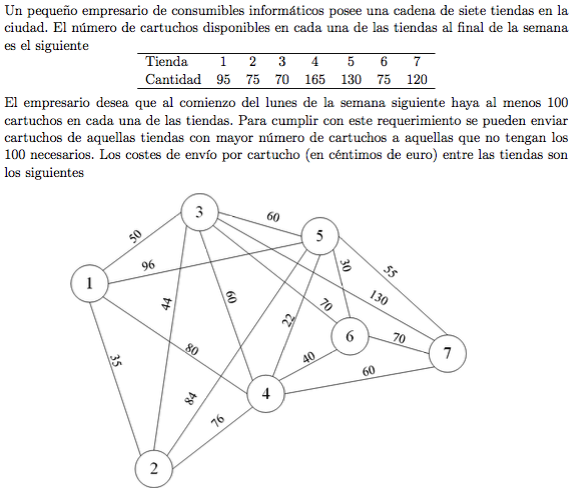
\includegraphics[width=0.75\textwidth]{res/Exercise_1.png}
        \end{figure}

		\subsection{Determinar la mejor manera de distribuir los cartuchos entre las tiendas.}

			\paragraph{}


		\subsection{?`En cuánto puede variar el coste de eníoo entre las tiendas 4 y 6 para que la solución Óptima calculada en el apartado (a) se mantenga? Razonar la respuesta.}

			\paragraph{}


		\subsection{Sin realizar iteraciones, obtener la nueva solución si el número de cartuchos disponibles en la tienda número 3 disminuye a 65 y el de la tienda 5 aumenta a 135 unidades. Justificar la respuesta.}

			\paragraph{}


		\subsection{Escribir el problema dual del formulado en el apartado (a)}

			\paragraph{}


		\subsection{Resolver el problema del apartado (e) utilizando las condiciones de holgura complementaria. ?`Es única la solución? Razonar la respuesta.}

			\paragraph{}


		\subsection{Suponer ahora que los cartuchos se pueden enviar entre todas las tiendas conectadas. Modelizar, sin resolver, este nuevo problema.}

			\paragraph{}


    \section{Ejercicio 2}

        \begin{figure}[H]
        \centering
            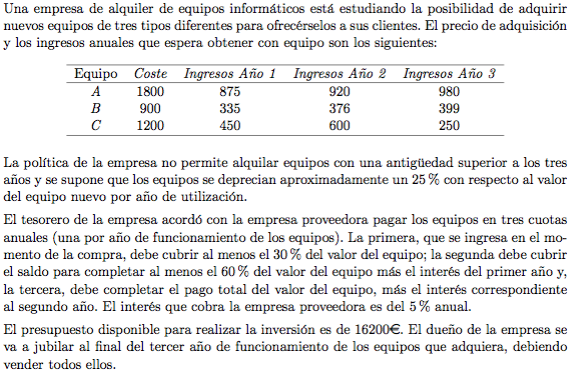
\includegraphics[width=0.75\textwidth]{res/Exercise_2.png}
        \end{figure}

		\subsection{Formular un modelo de PL para determinar el plan Óptimo de compras y de pagos que maximice los beneficios al final del periodo de tres años.}

			\paragraph{}


		\subsection{?`Cuál es el plan Óptimo?}

			\paragraph{}


		\subsection{Escribir el problema dual del formulado en el apartado (a).}

			\paragraph{}


		\subsection{Determinar la solución Óptima del problema formulado en (c) utilizando las condiciones de holgura complementaria.}

			\paragraph{}


		\subsection{Interpretar la variable dual asociada a la restricción del presupuesto disponible.}

			\paragraph{}


\end{document}
